\begin{frame}{2. Neural Networks Structure}
In this work, we aim to optimize the following loss function
\begin{align}
    \mathcal{L}=\frac{1}{M}\sum_{n=1}^{M}\left( \hat{G} * F_n -U_n\right)^2 + \lambda\left( \displaystyle \Delta(\hat{G} * F_n)  - F_n \right)^2,
\end{align}
where $\hat{G}$ is the predict Green's function by NN, $*$ is the numerical integration, $\displaystyle \Delta$ is the Laplacian computed by differential matrix and $\lambda$ is a parameter controlled the PDE loss.
$U_n$ and $F_n$ are the value generated by
\begin{align}
    U_n&=\sum_{(k_1, k_2) \in \Omega_K} \alpha_{k_1, k_2} \sin{\Bigl( \frac{k_1\pi(X+1)}{2} \Bigr)}\sin{\Bigl( \frac{k_2\pi(Y+1)}{2} \Bigr)},\\
    F_n&=\sum_{(k_1, k_2) \in \Omega_K} \alpha_{k_1, k_2} \Bigl( - \bigl( \frac{k_1\pi}{2} \bigr)^2 - \bigl( \frac{k_2\pi}{2} \bigr)^2 \Bigr) \sin{\Bigl( \frac{k_1\pi(X+1)}{2} \Bigr)}\sin{\Bigl( \frac{k_2\pi(Y+1)}{2} \Bigr)},
\end{align} 
where $\Omega_K$ is a finite set of frequency pairs $(k_1, k_2)$ randomly sampled from $\mathbb{N}^2$ for each sample $n$,
 and $\alpha_{k_1, k_2}$ represents the randomly generated coefficients and $X, Y$ are 2D grid points. 
\end{frame}



\begin{frame}
    \begin{columns}[T]
    
    \begin{column}{0.44\textwidth}
        \textbf{Plan A:}
        \begin{figure}
            \centering
            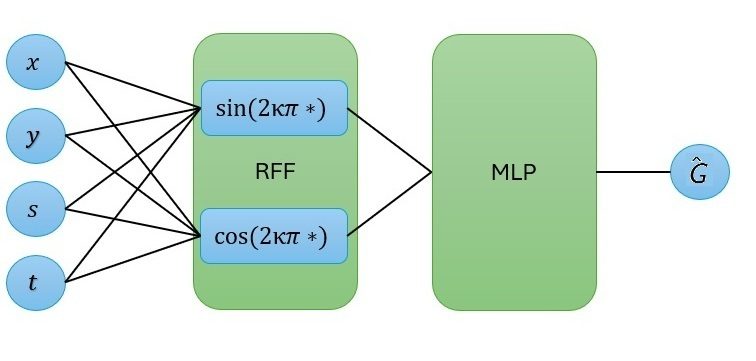
\includegraphics[width=\linewidth]{imgs/NNstructureB.jpg}
        \end{figure}
        \begin{itemize}
            \item Input: $(x,y,s,t) \Rightarrow N^4$
            \item Size of training data: $M \cdot N^4$
        \end{itemize}
    \end{column}
    \hfill
    \begin{column}{0.44\textwidth}
        \textbf{Plan B:}
        \begin{figure}
            \centering
            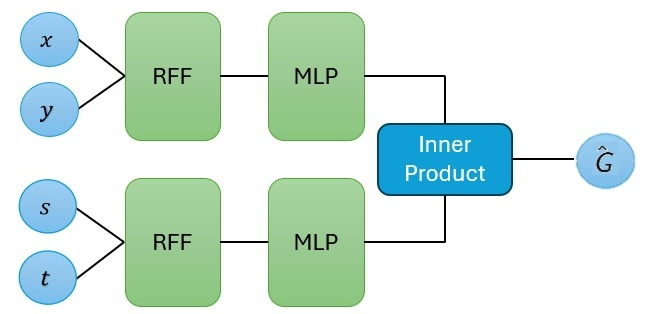
\includegraphics[width=\linewidth]{imgs/NNstructureA.jpg}
        \end{figure}
        \begin{itemize}
            \item Input: $(x,y)$ \& $(s,t) \Rightarrow 2N^2$
            \item Size of training data: $M \cdot 2N^2$
        \end{itemize}
    \end{column}

\end{columns}
\vspace{1em}
Since the size of the input vector determines the training time, we try to decrease it.
 We employ two separate networks and compute the inner product of their output vectors, which mimics the separation of variables in Plan B.

\end{frame}